\documentclass[a4paper, 10pt]{article}
\usepackage{physics}
\usepackage{tikz}
\usepackage{tikz-3dplot}
\usepackage[outline]{contour} % glow around text
\usepackage{xcolor}

% Encoding
\usepackage[T1]{fontenc}
\usepackage[utf8]{inputenc}
\usepackage[english]{babel}

% Margins
\usepackage[left=2.5cm, right=2.5cm]{geometry}

% Mathematics
\usepackage{amsmath, amssymb, mathtools, amsthm}

% Bibliography (uncomment if needed)
\usepackage{csquotes}
\usepackage[backend=biber, sorting=none, style=nature]{biblatex}
\addbibresource{biblio.bib}

% Tikz
\usepackage{tikz}
\usetikzlibrary{math}

% Personal taste
\usepackage[font=footnotesize]{caption}
\usepackage[parfill]{parskip}

% Theorems
\newtheorem{theorem}{Theorem}
\newtheorem{lemma}{Lemma}

% Commands
\newcommand{\rn}{\mathbb{R}^n}
\newcommand{\SN}{S^{n-1}}
\newcommand{\PN}{P^{n-1}}
\newcommand{\pack}{\text{pack}_{\alpha}}
\newcommand{\cov}{\text{cov}_{\alpha}}

\title{Quasi-orthogonality notes}
\author{}

\begin{document}

  \maketitle

  \section{Preliminaries}
  We take everything from \cite{kainen1992}. Here are the definitions:
  
  \begin{enumerate}
    \item On the sphere $\SN = \{x \in R^n : ||x|| = 1\}$, we define the
      \textbf{angle metric} defined as $\angle(x,y) = \arccos(x\cdot y)$. With
      respect to this metric, $\SN$ has diameter $\pi$. By definition,
      $\angle{x,-y} := \angle{-x,y}$;
    \item define the \textbf{elliptic space} $\PN$ as the set of all
      unordered antipodal pairs in $S^{n-1}$. Here we define a similar metric,
      namely $\angle(x,y) = \min\{\angle(x,y), \angle(-x,y) \}$. The diameter of
      $\PN$ is therefore $\pi/2$;
    \item we call \textbf{spherical (elliptical) code} a subset of $\SN$
      $(\PN)$;
    \item for any \textbf{finite subset $X$} of $\SN$, the \textbf{skewness of
      $X$} is the non-negative number
      $$ \mu(X) := \sup\{|x \cdot y| : x \neq y \in X\}$$
      One can see that $X$ contains antipodes if and only if $\mu(X) = 1$, and
      is strictly orthogonal if and only if $\mu(X) = 0$;
    \item we call $X$ \textbf{$\epsilon$-orthogonal} if $\mu(X) < \epsilon$;
    \item for any $A \in \SN$, the \textbf{$\epsilon$-dimension}
      $\dim_{\epsilon}(A)$ of $A$ is the larges number of elements in an
      $\epsilon$-orthogonal $X \subseteq A$.
  \end{enumerate}

  Apparently it is now easy to see the following consequences:

  \begin{lemma}
    For $n\geq 2$, and $\epsilon \in (0,1)$, if $d$ is the cardinality of the
    largest set $Y \subset \rn $ of non-zero vectors for which $y\neq u$ implies
    $|y \cdot u | < \epsilon ||y|| \, ||u||$, then $d = \dim_{\epsilon}(\SN)$.
  \end{lemma}

  \begin{lemma}
    For $n\geq 2$, and $\epsilon \in (0,1)$, if $d$ is the cardinality of the
    largest set $Y \subset \PN $ of non-zero vectors for which $y\neq u$ implies
    $\angle(y,u) \geq \arccos(\epsilon) $, then $d = \dim_{\epsilon}(\SN)$.
  \end{lemma}

  We continue with some more definitions:
  \begin{enumerate}
    \item an \textbf{isometry} between metric spaces is a map $\omega: E
      \rightarrow E'$ for which holds that $h'(\omega(x), \omega(y)) = h(x,y)$,
      where $h$ and $h'$ are the distances on $E$ and $E'$;
    \item a \textbf{segment from $x$ to $y$} is an isometry of a real interval
      $[a,b]$ onto $E$ so that $\omega(a) = x$ and $\omega(b) = y$.
    \item a metric space is \textbf{excellent} if for any two points there is a
      segment joining them. \textbf{Assume for now that all metric spaces are
      excellent}.
  \end{enumerate}
  
  Introducing the neighbourhoods:

  \begin{enumerate}
    \item for some $\alpha>0$ and $s \in E$ we define the \textbf{closed
      $\alpha$-neighbourhood} $N_{\alpha}(s) = \{x\in E : h(x,s) < \alpha\}$;
    \item We call a neighbourhood \textbf{a cap} if we are working on a sphere
      (since the distance is defined as the arc distance I guess);
    \item we can define the neighbourhood of a subset as the set of point
      neighbourhoods;
  \end{enumerate}

  Some more general definitions:
  \begin{enumerate}
    \item for any metric space $(E,h)$, we say that a subset $T \subseteq E$ is
      \textbf{$s$-separated} if for all $t,t' \in T$ we have that $h(t,t') > s$.
    \item a family $\mathcal{F}$ of sets $F \subset E$ is a \textbf{packing of
      $E$} if for all $F \neq F'$, $F \cap F' = \varnothing$;
    \item a family $\mathcal{F}$ of sets $F \subset E$ is a \textbf{covering of
      $E$} if $E = \bigcup\{F : F \in \mathcal{F}\}$;
  \end{enumerate}

  Now a bit more specific:
  \begin{enumerate}
    \item we call $T$ an \textbf{$\alpha$-packing (covering)} if $N_{\alpha}(T)$
      is a packing (covering). We see that $T$ is $\alpha$-separated precisely
      when it is an $\alpha/2$-packing.
  \end{enumerate}

  More specifically on packings:
  \begin{enumerate}
    \item we write $\pack(E)$ for the largest number of elements in any
      $\alpha$-packing;
    \item we call an $\alpha$-packing $T$ \textbf{maximal} if $T \cup \{x\}$ is
      not an $\alpha$-packing, if $x \notin T$;
    \item we call an $\alpha$-packing $T$ \textbf{maximum} if no other packing
      has more elements.
  \end{enumerate}

  Similarly for coverings:
  \begin{enumerate}
    \item we write $\cov(E)$ for the smallest number of elements in any
      $\alpha$-covering;
    \item we call an $\alpha$-covering $T$ \textbf{minimal} if no subset is an
      $\alpha-cover$;
    \item we call an $\alpha$-covering $T$ \textbf{minimum} if no other covering
      has fewer elements.
  \end{enumerate}

  \begin{figure}
    \begin{tikzpicture}
      \draw (0,0) circle (2);
      \draw (0,0) -- (0:2);
      \draw[fill=black] (0:2) circle (2pt);
      \node[font=\large] at (0:2.5){$y$};
      \draw[fill=black] (110:2) circle (2pt);
      \draw (0,0) -- (110:2);
      \node[font=\large] at (110:2.5){$u$};
    \end{tikzpicture}
  \end{figure}

  \begin{figure}
    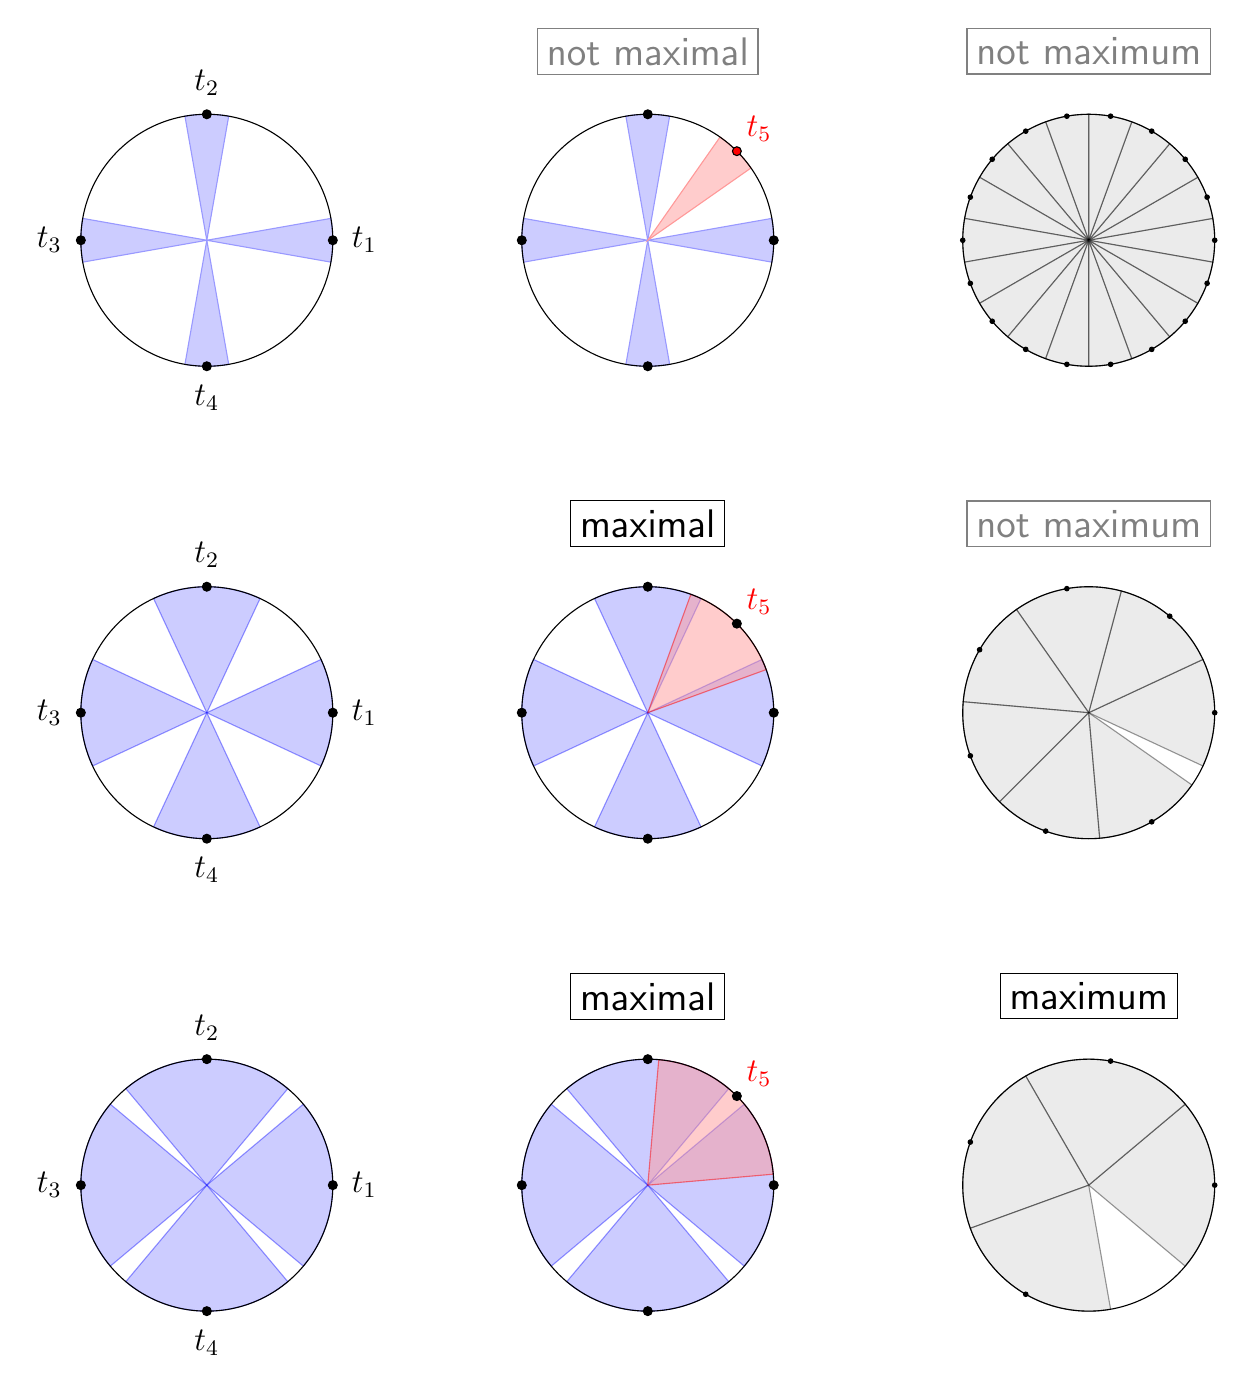
\begin{tikzpicture}

  % Upper row
  \begin{scope}

    % Left fiure
    \begin{scope}[scale=0.8]
      \foreach \i/\th in {1/0, 2/90, 3/180, 4/270} {

        \filldraw[fill=blue!20, draw=blue!40] (0,0)
          -- (\th-10:2)
          arc [start angle=\th-10, end angle=\th+10, radius=2]
          -- cycle;

        \draw[fill=black] (\th:2) circle (2pt);
        \node[font=\large] at (\th:2.5){$t_{\i}$};
      }
      \draw (0,0) circle (2);
      % \node[color=blue, font=\Large] at (0,3.5) {$\alpha=10^{\circ}$};
    \end{scope}

    % Center figure
    \begin{scope}[scale=0.8, xshift=7cm]
      \foreach \i/\th in {1/0, 2/90, 3/180, 4/270} {

        \filldraw[fill=blue!20, draw=blue!40] (0,0)
          -- (\th-10:2)
          arc [start angle=\th-10, end angle=\th+10, radius=2]
          -- cycle;

        \draw[fill=black] (\th:2) circle (2pt);
        % \node[font=\large] at (\th:2.5){$t_{\i}$};
      }

      \filldraw[fill=red!20, draw=red!40] (0,0)
        -- (35:2)
        arc [start angle=35, end angle=55, radius=2]
        -- cycle;

      \draw (0,0) circle (2);
      \draw[fill=red] (45:2) circle (2pt);
      \node[font=\large, color=red] at (45:2.5){$t_{5}$};
      \node[font=\Large\sffamily, draw, color=black!50] at (0,3) {not maximal};

    \end{scope}

    % Right figure
    \begin{scope}[scale=0.8, xshift=14cm]
      \foreach \th in {0,20,...,340} {
        \filldraw[fill=gray!40, draw=black, opacity=0.4] (0,0)
          -- (\th-10:2)
          arc [start angle=\th-10, end angle=\th+10, radius=2]
          -- cycle;
        \draw[fill=black] (\th:2) circle (1pt);
      }
      \draw (0,0) circle (2);
      \node[font=\Large\sffamily, draw, color=black!50] at (0,3) {not maximum};
    \end{scope}
  \end{scope}


  % Middle row 
  \begin{scope}[yshift=-6cm]

    % Left figure
    \begin{scope}[scale=0.8]
      \foreach \i/\th in {1/0, 2/90, 3/180, 4/270} {

        \filldraw[fill=blue!50, draw=blue, opacity=0.4] (0,0)
          -- (\th-25:2)
          arc [start angle=\th-25, end angle=\th+25, radius=2]
          -- cycle;

        \draw[fill=black] (\th:2) circle (2pt);
        \node[font=\large] at (\th:2.5){$t_{\i}$};
      }
      \draw (0,0) circle (2);
    \end{scope}

    % Middle fig
    \begin{scope}[scale=0.8, xshift=7cm]
      \foreach \i/\th in {1/0, 2/90, 3/180, 4/270} {

        \filldraw[fill=blue!50, draw=blue, opacity=0.4] (0,0)
          -- (\th-25:2)
          arc [start angle=\th-25, end angle=\th+25, radius=2]
          -- cycle;

        \draw[fill=black] (\th:2) circle (2pt);
        % \node[font=\large] at (\th:2.5){$t_{\i}$};
      }

      \filldraw[fill=red!40, draw=red, opacity=0.5] (0,0)
        -- (20:2)
        arc [start angle=20, end angle=70, radius=2]
        -- cycle;

      \draw[fill=black] (45:2) circle (2pt);
      \node[font=\large, color=red] at (45:2.5){$t_{5}$};

      \draw (0,0) circle (2);
      \node[font=\Large\sffamily, draw] at (0,3) {maximal};
    \end{scope}

    % Right fig
    \begin{scope}[scale=0.8, xshift=14cm]
      \foreach \th in {0,50,...,300} {
        \filldraw[fill=gray!40, draw=black, opacity=0.4] (0,0)
          -- (\th-25:2)
          arc [start angle=\th-25, end angle=\th+25, radius=2]
          -- cycle;
        \draw[fill=black] (\th:2) circle (1pt);
      }
      \draw (0,0) circle (2);
      \node[font=\Large\sffamily, draw, color=black!50] at (0,3) {not maximum};
    \end{scope}
  \end{scope}

  % Bottom row 
  \begin{scope}[yshift=-12cm]

    % Left figure
    \begin{scope}[scale=0.8]
      \foreach \i/\th in {1/0, 2/90, 3/180, 4/270} {

        \filldraw[fill=blue!50, draw=blue, opacity=0.4] (0,0)
          -- (\th-40:2)
          arc [start angle=\th-40, end angle=\th+40, radius=2]
          -- cycle;

        \draw[fill=black] (\th:2) circle (2pt);
        \node[font=\large] at (\th:2.5){$t_{\i}$};
      }
      \draw (0,0) circle (2);
      % \node[font=\Large, color=blue] at (0,3.5) {$\alpha=30^{\circ}$};
    \end{scope}

    % Middle fig
    \begin{scope}[scale=0.8, xshift=7cm]
      \foreach \i/\th in {1/0, 2/90, 3/180, 4/270} {

        \filldraw[fill=blue!50, draw=blue, opacity=0.4] (0,0)
          -- (\th-40:2)
          arc [start angle=\th-40, end angle=\th+40, radius=2]
          -- cycle;

        \draw[fill=black] (\th:2) circle (2pt);
        % \node[font=\large] at (\th:2.5){$t_{\i}$};
      }

      \filldraw[fill=red!40, draw=red, opacity=0.5] (0,0)
        -- (5:2)
        arc [start angle=5, end angle=85, radius=2]
        -- cycle;

      \draw[fill=black] (45:2) circle (2pt);
      \node[font=\large, color=red] at (45:2.5){$t_{5}$};

      \draw (0,0) circle (2);
      \node[font=\Large\sffamily, draw, color=black] at (0,3) {maximal};
    \end{scope}

    % Right fig
    \begin{scope}[scale=0.8, xshift=14cm]
      \foreach \th in {0,80,...,240} {
        \filldraw[fill=gray!40, draw=black, opacity=0.4] (0,0)
          -- (\th-40:2)
          arc [start angle=\th-40, end angle=\th+40, radius=2]
          -- cycle;
        \draw[fill=black] (\th:2) circle (1pt);
      }
      \draw (0,0) circle (2);
      \node[font=\Large\sffamily, draw] at (0,3) {maximum};
    \end{scope}
  \end{scope}
\end{tikzpicture}


  \end{figure}

  Now the main theorem:
  \begin{theorem}
    For any $\epsilon \in (0,1)$, $\dim_{\epsilon}(\PN) = \pack(\PN)$, where
    $\alpha = \frac{1}{2}\arccos(\epsilon)$.
  \end{theorem}

  \begin{figure}
    % Author: Izaak Neutelings (June 2017)
% taken from https://tex.stackexchange.com/questions/159445/draw-in-cylindrical-and-spherical-coordinates
% \documentclass[border=3pt,tikz]{standalone}
% \usepackage{physics}
% \usepackage{tikz}
% \usepackage{tikz-3dplot}
% \usepackage[outline]{contour} % glow around text
% \usepackage{xcolor}

\colorlet{veccol}{green!50!black}
\colorlet{projcol}{blue!70!black}
\colorlet{myblue}{blue!80!black}
\colorlet{myred}{red!90!black}
\colorlet{mydarkblue}{blue!50!black}
\tikzset{>=latex} % for LaTeX arrow head
\tikzstyle{proj}=[projcol!80,line width=0.08] %very thin
\tikzstyle{area}=[draw=veccol,fill=veccol!80,fill opacity=0.6]
\tikzstyle{vector}=[-stealth,myblue,thick,line cap=round]
\tikzstyle{unit vector}=[->,veccol,thick,line cap=round]
\tikzstyle{dark unit vector}=[unit vector,veccol!70!black]
\contourlength{1.3pt}

% 3D AXIS with spherical coordinates, dA
\tdplotsetmaincoords{60}{103}
\begin{tikzpicture}[scale=2.8,tdplot_main_coords]
  
  % VARIABLE
  \def\rvec{1.0}
  \def\thetavec{35}
  \def\phivec{45}
  \def\dtheta{10}
  \def\dphi{16}
  \def\sphere#1#2#3{plot[domain=#1]({\rvec*sin(#2)*cos(#3)},{\rvec*sin(#2)*sin(#3)},{\rvec*cos(#2)})}
  \contourlength{0.8pt}
  
  % AXES
  \coordinate (O) at (0,0,0);
  % \draw[thick,->] (0,0,0) -- (1.16*\rvec,0,0) node[left=2,below]{$x$};
  % \draw[thick,->] (0,0,0) -- (0,1.1*\rvec,0) node[below=2,right=0]{$y$};
  % \draw[thick,->] (0,0,0) -- (0,0,1.1*\rvec) node[above]{$z$};
  
  % COORDINATES
  \tdplotsetcoord{P}{\rvec}{\thetavec}{\phivec}
  \tdplotsetcoord{PB}{\rvec}{\thetavec+\dtheta}{\phivec}
  \tdplotsetcoord{PR}{\rvec}{\thetavec}{\phivec+\dphi}
  \tdplotsetcoord{PBR}{\rvec}{\thetavec+\dtheta}{\phivec+\dphi}
  
  
  % PROJECTIONS
  \draw[proj] %\thetavec+\dtheta
    plot[domain=0:90]({\rvec*sin(\x)*cos(\phivec)},{\rvec*sin(\x)*sin(\phivec)},{\rvec*cos(\x)}) coordinate (BL);
  \draw[proj]
    plot[domain=0:90]({\rvec*sin(\x)*cos(\phivec+\dphi)},{\rvec*sin(\x)*sin(\phivec+\dphi)},{\rvec*cos(\x)}) coordinate (BR);
  \draw[proj]
    plot[domain=0:90]({\rvec*cos(\x)},{\rvec*sin(\x)},0);
  % \draw[proj] (O)  -- (BL); % PBxy
  % \draw[proj] (O)  -- (BR); % PBRxy
  % \draw[proj] (P)  -- (Pz);
  % \draw[proj] (PR)  -- (Pz) node[midway,above=-2,rotate=-24] {\contour{white}{$r\sin\theta$}};
  
\end{tikzpicture}


  \end{figure}
  \printbibliography


\end{document}
